% Laporan Tugas Workshop Deep Learning — Duta Rizky Pratama (124400027), Kelas RA, Lokasi 7.
% Compile: python ../buat_tabel.py  (setelah hasil/ablasi.csv lengkap), lalu latexmk -pdf main.tex
% Semua angka bersumber dari hasil/ablasi.csv (via buat_tabel.py). Teks merah \isi{...} = isian manual (perangkat, username GitHub); hapus sebelum kumpul.
\documentclass[conference,a4paper]{IEEEtran}
\IEEEoverridecommandlockouts
\usepackage[indonesian]{babel}
\usepackage[utf8]{inputenc}
\usepackage[T1]{fontenc}
\usepackage{cite}
\usepackage{amsmath,amssymb}
\usepackage{graphicx}
\usepackage{booktabs}
\usepackage{multirow}
\usepackage{xcolor}
\usepackage[hidelinks]{hyperref}
\graphicspath{{gambar/}{hasil/}}
\newcommand{\isi}[1]{\textcolor{red}{[#1]}}
\newcommand{\tabel}[1]{\InputIfFileExists{hasil/tabel/#1.tex}{}{\isi{tabel #1 belum dibuat: jalankan buat\_tabel.py}}}
\InputIfFileExists{hasil/tabel/makro.tex}{}{\newcommand{\totalmenit}{\isi{x}}\newcommand{\jumlahrun}{\isi{n}}}

\begin{document}
\title{Studi Ablasi RNN, LSTM, dan GRU dibandingkan ANN untuk Prediksi Trafik Seluler Kota Milan}
\author{\IEEEauthorblockN{Duta Rizky Pratama}
\IEEEauthorblockA{NIM 124400027 \textbullet\ Kelas RA\\
Teknik Telekomunikasi, ITERA\\
Lokasi kelompok: Universit\`a Bicocca (kode 7, kotak 7467)}}
\maketitle

\begin{abstract}
Operator seluler perlu meramal trafik per sel agar sumber daya dapat disiapkan lebih awal. Studi ini membandingkan ANN, RNN, LSTM, dan GRU untuk prediksi aktivitas internet satu jam ke depan pada data Telecom Italia (Duomo dan Universit\`a Bicocca) melalui studi ablasi: lima faktor wajib dan dua faktor pilihan (\textit{batch size}, dropout), masing-masing diubah satu per satu dengan tiga seed. Pada konfigurasi acuan, RNN dan GRU terbaik (test MAE $230\pm5$ dan $237\pm9$), diikuti LSTM ($274\pm25$) dan ANN ($310\pm6$); semuanya mengalahkan baseline naif terbaik (468). \textit{Learning rate}, jumlah lapisan (LSTM), dropout (ANN), dan panjang jendela (ANN) paling berpengaruh, sedangkan dropout justru merugikan semua model. Menggabungkan nilai terbaik tiap faktor hanya menurunkan val MAE ANN ($-14{,}5\%$); pada RNN, LSTM, dan GRU gabungan itu lebih buruk dari acuan pada validasi karena interaksi antar faktor. Di Bicocca selisih antar model mengecil hingga setara derau seed, dan pada minggu Natal semua model kalah jauh dari tebakan naif ``nilai terakhir''.
\end{abstract}
\begin{IEEEkeywords}
prediksi trafik seluler, RNN, LSTM, GRU, studi ablasi
\end{IEEEkeywords}

\section{Pendahuluan}
Peramalan trafik per sel mendukung penjadwalan sumber daya radio, penghematan energi, dan perencanaan kapasitas. Trafik seluler berpola harian dan mingguan, sehingga model yang membaca urutan, yaitu RNN, LSTM \cite{hochreiter1997lstm}, dan GRU \cite{cho2014gru}, lazim dibandingkan dengan jaringan umpan-maju (ANN) yang memperlakukan jendela masukan sebagai vektor datar. Membandingkan satu konfigurasi saja dapat menyesatkan karena peringkat model bisa berubah mengikuti hyperparameter. Studi ablasi mengubah satu faktor dalam satu waktu sehingga pengaruhnya terpisah. Kontribusi: (i) ablasi tujuh faktor untuk empat model dengan tiga seed; (ii) pemilihan konfigurasi terbaik yang jujur (val MAE) beserta pengujiannya pada minggu test dan Natal; (iii) uji generalisasi ke lokasi dengan pola trafik berbeda.

\section{Data dan Metode}
\subsection{Dataset}
Data berasal dari Telecom Italia Big Data Challenge \cite{barlacchi2015milan} dalam versi per jam \cite{zhang2021fedda}, 4 November--29 Desember 2013, dengan fitur \textit{net} (aktivitas internet, target), \textit{call}, dan \textit{sms}. Lokasi utama adalah Duomo (kotak 5060); lokasi kelompok adalah Universit\`a Bicocca (kode 7, kotak 7467), kampus di pinggir kota (Gambar~\ref{fig:peta}).
\begin{figure}[t]
  \centering
  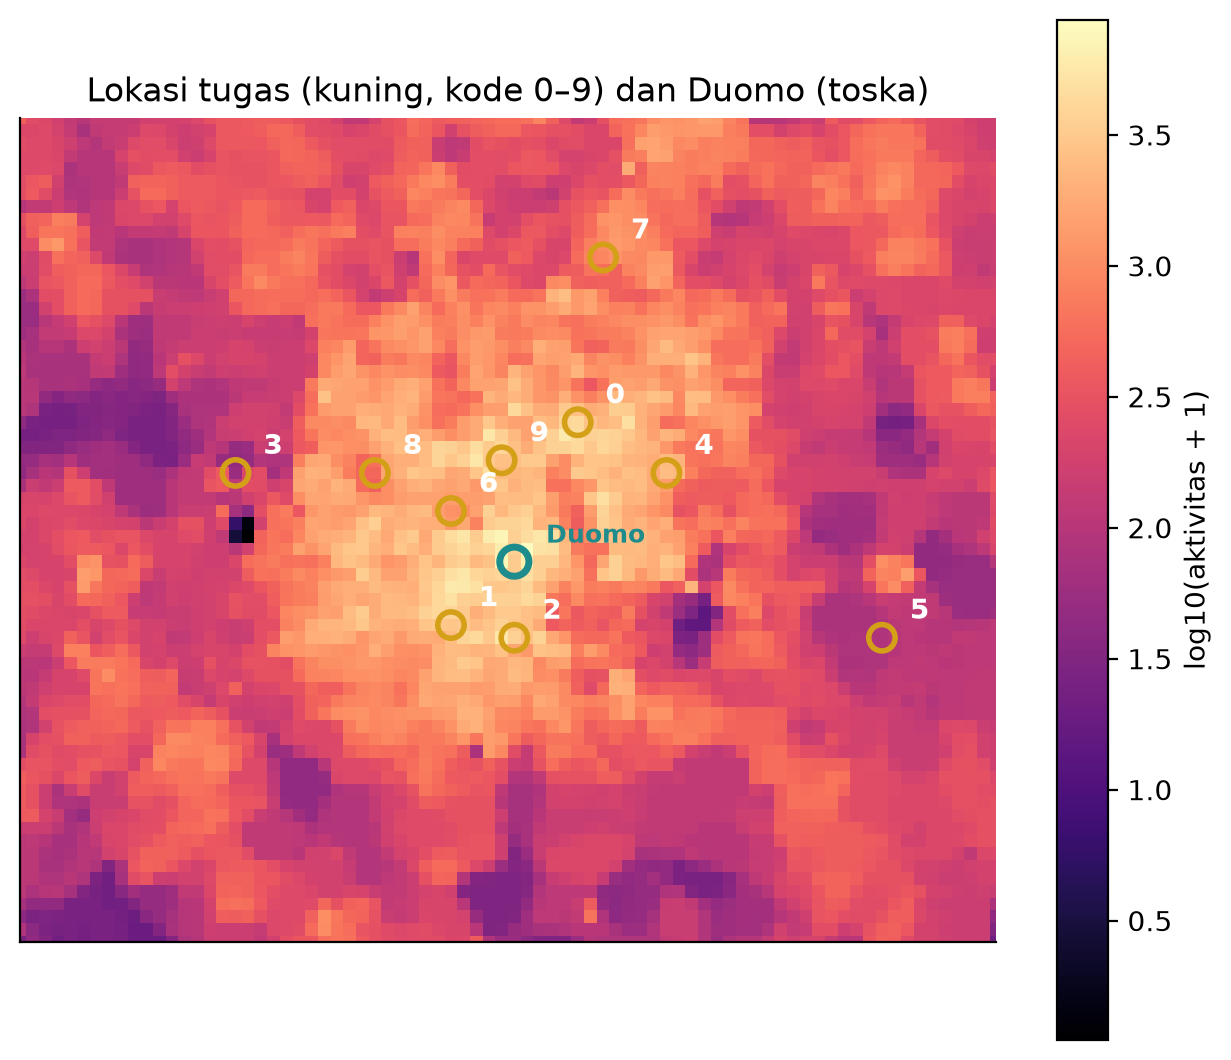
\includegraphics[width=0.78\linewidth]{peta_lokasi_tugas.png}
  \caption{Rata-rata aktivitas internet per kotak di Milan; kuning: lokasi tugas, toska: Duomo.}
  \label{fig:peta}
\end{figure}

\subsection{Pembagian Data dan Praproses}
Pembagian berdasarkan waktu: train 11 Nov--8 Des, val 9--15 Des, test 16--22 Des, Natal 23--29 Des; minggu pertama hanya konteks jendela. Data tidak diacak karena sampel berdekatan berkorelasi kuat; pengacakan membocorkan informasi masa depan ke data latih dan membuat galat tampak terlalu kecil. Standarisasi memakai statistik sebelum minggu validasi. Sampel dibentuk dengan jendela geser $W$ jam untuk meramal jam berikutnya (672 sampel latih pada $W{=}24$). Implementasi memakai PyTorch \cite{paszke2019pytorch}.

\subsection{Model dan Konfigurasi Acuan}
ANN meratakan jendela $[W,\text{fitur}]$ lalu melewatkannya pada lapisan tersembunyi ReLU. RNN, LSTM, dan GRU memproses jendela langkah demi langkah dan memakai \textit{hidden state} jam terakhir untuk lapisan keluaran. RNN polos hanya punya satu transformasi per langkah; LSTM menambah sel memori dan tiga gerbang; GRU memakai dua gerbang. Ukuran hidden acuan (ANN 32, RNN 68, LSTM 33, GRU 38) dipilih agar parameter model rekuren sama ($\approx$5,5 ribu). Acuan: $W{=}24$, horizon 1 jam, ANN 2 lapisan dan rekuren 1 lapisan, 7 fitur (net, call, sms, jam dan hari sinus-kosinus), Adam \textit{lr} $10^{-3}$, batch 64, MSE, \textit{early stopping} \textit{patience} 30 (maks.\ 300 epoch), tanpa dropout dan \textit{clipping}.

\subsection{Protokol Ablasi dan Evaluasi}
Faktor wajib: A1 $W\in\{6,12,24,48,168\}$; A2 hidden $\in\{16,32,64,128\}$; A3 lapisan $\in\{1,2,3\}$; A4 \textit{lr} $\in\{10^{-4},10^{-3},10^{-2}\}$; A5 fitur $\in$ \{net, net+call+sms, net+waktu, semua\}. Faktor pilihan: B1 \textit{batch} $\in\{16,64,256\}$ dan B2 dropout $\in\{0;0{,}2;0{,}5\}$. Setiap konfigurasi dilatih dengan seed 0, 1, 2 dan dilaporkan sebagai rerata$\pm$simpangan baku (sd). Metrik: MAE, RMSE, MAPE pada skala asli. Konfigurasi terbaik dipilih dengan val MAE saja; minggu test dan Natal hanya untuk pelaporan akhir. Perangkat: Google Colab (GPU NVIDIA T4); \jumlahrun\ run tercatat dengan total waktu training $\approx$ \totalmenit\ menit. Semua angka dapat dilacak ke \texttt{hasil/ablasi.csv}.

\emph{Hipotesis B (ditulis sebelum menjalankan).} B1: batch 16 terbaik karena sekitar 42 pembaruan per epoch (vs.\ sekitar 3 untuk batch 256) pada 672 sampel dan derau gradien berfungsi sebagai regularisasi ringan; batch 256 paling lambat konvergen. B2: dropout 0,2 sedikit membantu ANN dan model besar, sedangkan 0,5 merugikan model rekuren kecil karena \textit{underfitting} dan menaikkan sd antar seed. Kedua faktor dipilih karena pada data sekecil ini jumlah pembaruan dan regularisasi diduga paling menentukan.

\section{Hasil dan Pembahasan}
\subsection{Bagian 0: Baseline Naif dan Acuan}
\tabel{tab_naif}
Di Duomo, tebakan naif terbaik pada minggu test adalah ``minggu lalu'' (MAE 468); semua model acuan lebih baik (Tabel~\ref{tab:C}, baris acuan): RNN $230\pm5$, GRU $237\pm9$, LSTM $274\pm25$, ANN $310\pm6$, sesuai nilai referensi Sesi 2 (ANN $\approx$310, RNN $\approx$230, LSTM $\approx$274, GRU $\approx$237). Selisih RNN dan GRU lebih kecil daripada sd antar seed sehingga keduanya tidak dapat dibedakan; ANN jelas paling buruk dan LSTM tidak stabil antar seed (sd 25). Keunggulan RNN/GRU atas ANN sesuai dengan sifat modelnya: bobot dipakai bersama sepanjang waktu sehingga jumlah parameter tetap kecil, sedangkan ANN harus mempelajari bobot terpisah untuk tiap jam dalam jendela. Pada minggu Natal situasinya berbalik: ``minggu lalu'' memburuk (1426) karena pola libur menyimpang dari minggu kerja, dan ``nilai terakhir'' (431) hanya disamai RNN (421$\pm$2), sedangkan GRU (468), LSTM (586), dan ANN (680) lebih buruk.

\subsection{Bagian A dan B: Ablasi}
\tabel{tab_AB}
\begin{figure*}[t]
  \centering
  \IfFileExists{hasil/fig_A.png}{\includegraphics[width=\textwidth]{fig_A.png}}{\isi{fig\_A.png belum dibuat}}
  \caption{MAE val (atas) dan test (bawah) terhadap nilai tiap faktor A1--A5; area = $\pm1$ sd.}
  \label{fig:A}
\end{figure*}
Tabel~\ref{tab:AB}, Gambar~\ref{fig:A}, dan Tabel~\ref{tab:sens} merangkum seluruh ablasi.

\textbf{A1 (jendela).} ANN paling sensitif: val MAE naik dari 212 ($W{=}6$) menjadi 298 ($W{=}168$) dan test dari 269 menjadi 402, sementara parameternya membengkak dari 2,5 ribu menjadi 38,8 ribu dan epoch berhenti makin cepat (167 $\to$ 76). Dengan 672 sampel latih, lapisan pertama berukuran $W{\times}7{\times}32$ menghafal alih-alih menggeneralisasi, dan ANN tidak punya bias urutan untuk memanfaatkan jam-jam lama. RNN dan GRU hampir datar (rentang val 15 dan 6) karena parameter mereka tidak bergantung pada $W$ dan \textit{hidden state} meringkas konteks; jendela panjang tidak menolong, mungkin karena informasi paling relevan untuk horizon 1 jam ada pada beberapa jam terakhir ditambah fitur waktu. Pada $W{=}6$ ANN (212) setara RNN (216), menunjukkan jendela panjang hanya menguntungkan model yang membaca urutan.

\textbf{A2 (hidden).} Model lebih besar tidak overfit secara merugikan: GRU turun dari 217 ke 189 dan LSTM dari 244 ke 207 (val) seiring hidden 16$\to$128, kemungkinan karena \textit{early stopping} sudah berperan sebagai regularisasi. RNN jenuh pada hidden 64 (207 vs.\ 208 pada 128, dengan parameter 4,7 ribu vs.\ 17,7 ribu). Dengan hidden sama jumlah parameter tidak setara (hidden 128: LSTM 70 ribu, GRU 53 ribu, RNN 18 ribu), sehingga perbandingan menurut parameter lebih adil: pada $\approx$4--5 ribu parameter, RNN (207) dan GRU (210) mengungguli LSTM (241), tetapi dengan kapasitas lebih besar GRU (189) melampaui RNN yang jenuh dan LSTM (207) menyamainya.

\textbf{A3 (lapisan).} Menumpuk lapisan tidak membantu dan merugikan LSTM: val 230 $\to$ 255 $\to$ 339 dan test 274 $\to$ 309 $\to$ 413 untuk 1/2/3 lapisan, dengan epoch menyusut. RNN juga memburuk pada 3 lapisan (225), GRU relatif tahan (203--212), ANN hampir tidak berubah (rentang 8). Parameter bertambah 3--4$\times$ pada data kecil, dan jalur gradien yang menembus beberapa lapisan rekuren sekaligus sepanjang waktu lebih sulit dioptimalkan; GRU dengan parameter lebih sedikit per lapisan dan gerbang lebih sederhana lebih toleran.

\textbf{A4 (\textit{learning rate}).} Pada $10^{-4}$ seluruh 12 run berhenti di batas 300 epoch (belum konvergen), sehingga rentang besar pada Tabel~\ref{tab:sens} (LSTM 183, GRU 191) sebagian besar artefak dari batas epoch, bukan sensitivitas intrinsik. Pembandingan yang bermakna adalah $10^{-3}$ vs.\ $10^{-2}$: LSTM membaik (val 230 $\to$ 216; test 274 $\to$ 226) dan GRU setara pada val (208) dengan test terbaik (216), sedangkan RNN (206 $\to$ 223) dan ANN (249 $\to$ 262) memburuk dengan sd lebih besar pada ANN (test $\pm$53). Gerbang LSTM/GRU menjaga aktivasi terbatas dan aliran gradien lebih stabil sehingga langkah besar masih aman, sedangkan RNN polos dan ANN lebih mudah melompati minimum; epoch turun ke $\approx$65 pada $10^{-2}$.

\textbf{A5 (fitur).} Hanya \textit{net} paling buruk bagi model rekuren pada val (RNN 245, LSTM 266, GRU 265 vs.\ 206--230 dengan fitur lengkap), jadi fitur tambahan berguna. Fitur waktu menyumbang paling besar: net+waktu mendekati \textit{semua} untuk ANN, LSTM, dan GRU (selisih $\le$6), sedangkan call/sms tanpa fitur waktu kurang berguna (kecuali pada RNN, yang setara); hanya RNN yang masih mengambil manfaat dari call/sms di atas waktu (223 $\to$ 206). ANN justru paling stabil terhadap fitur (rentang 12) dan pada test \textit{net} saja terbaik (272 vs.\ 310), indikasi bahwa fitur tambahan menambah dimensi masukan dan risiko overfit pada ANN, sedangkan model rekuren memanfaatkan fitur waktu untuk menebak posisi dalam siklus harian-mingguan.

\textbf{B1 (batch) --- hipotesis terbukti.} Batch 16 memberi val MAE terbaik atau setara untuk semua model (ANN 245, RNN 202, LSTM 209, GRU 202; LSTM turun 21 dari acuan) sedangkan batch 256 terburuk (RNN 228, LSTM 270). Pada batch 256 hanya sekitar 3 pembaruan per epoch; 5 dari 12 run menyentuh batas 300 epoch sebelum konvergen. Harganya: waktu per epoch sekitar 4$\times$ lebih lama pada batch 16 (mis.\ GRU 0,089 s vs.\ 0,024 s) dan total waktu run sekitar 2$\times$ batch 64, meski jumlah epoch lebih sedikit. LSTM paling sensitif (rentang 60), konsisten dengan keempat matriks gerbangnya yang membutuhkan lebih banyak pembaruan.

\textbf{B2 (dropout) --- hipotesis sebagian salah.} Dugaan bahwa dropout 0,5 merugikan model rekuren kecil benar (RNN 206 $\to$ 273), tetapi dugaan bahwa dropout 0,2 membantu ANN keliru: ANN justru paling terpukul (249 $\to$ 285 $\to$ 353, sd naik sampai $\pm$46). LSTM dan GRU hampir tidak terganggu pada 0,2 (+3 dan +4, dalam kisaran sd). Penjelasan: model ini tidak overfit berat karena \textit{early stopping} sudah menahannya, sehingga dropout hanya mengurangi kapasitas efektif; dropout sebelum lapisan keluaran pada regresi menambahkan derau pada prediksi (dua lapisan 32 neuron pada ANN kehilangan separuh unit pada 0,5).

\tabel{tab_sens}
\textbf{Ringkasan sensitivitas.} Setelah artefak $10^{-4}$ dikesampingkan, faktor paling berpengaruh bergantung pada model: dropout dan $W$ untuk ANN, jumlah lapisan dan batch untuk LSTM, dropout untuk RNN (67), dan fitur untuk GRU (57); jendela paling kecil pengaruhnya pada GRU dan RNN. Perbedaan antar model pada acuan (ANN vs.\ RNN: 80 pada test) lebih besar daripada sd seed (5--25), tetapi RNN vs.\ GRU tidak.

\subsection{Bagian C: Konfigurasi Terbaik}
Nilai terbaik tiap faktor dipilih dengan val MAE rata-rata lalu digabung (Tabel~\ref{tab:cfg}).
\tabel{tab_cfg}
\tabel{tab_C}
Penggabungan hanya memperbaiki val MAE ANN (249 $\to$ 213, $-14{,}5\%$; test 310 $\to$ 279, $-9{,}9\%$). Untuk RNN, LSTM, dan GRU, val MAE gabungan \emph{lebih buruk} dari acuan (214 vs.\ 206; 241 vs.\ 230; 227 vs.\ 208). Penyebabnya interaksi antar faktor: setiap nilai terbaik dicari sementara faktor lain tetap di acuan, lalu digabung menjadi model jauh lebih besar (GRU 152 ribu dan LSTM 70 ribu parameter, 13--28$\times$ acuan) dengan batch kecil yang mempercepat konvergen; epoch rata-rata turun menjadi 54--80 (dari 164--194), tanda overfit lebih awal. Konfigurasi gabungan GRU (hidden 128 dan 2 lapisan) bahkan lebih buruk daripada hanya mengubah hidden menjadi 128 (val 189). Pada test hasilnya campuran: LSTM membaik (274 $\to$ 247) dan GRU sedikit (237 $\to$ 230), RNN sedikit memburuk (230 $\to$ 242), padahal LSTM/GRU dengan \textit{lr} $10^{-2}$ saja (A4) mencapai test 226 dan 216, lebih baik daripada gabungan. Ini mengingatkan bahwa satu minggu validasi menjadi dasar pemilihan yang berderau (selisih val--test berubah arah antar model). Pada Natal, RNN (422) hanya setara ``nilai terakhir'' (431); model lain 442--563, sehingga tidak ada model yang andal pada pola libur karena data latih hanya memuat minggu kerja biasa. Sesuai aturan tugas, hasil ini dilaporkan apa adanya.

\subsection{Bagian D: Generalisasi di Universit\`a Bicocca}
\begin{figure}[t]
  \centering
  \IfFileExists{hasil/D_pola_lokasi.png}{\includegraphics[width=\linewidth]{D_pola_lokasi.png}}{\isi{D\_pola\_lokasi.png belum dibuat}}
  \caption{Pola aktivitas internet Duomo vs.\ Bicocca.}
  \label{fig:D}
\end{figure}
\tabel{tab_D}
Gambar~\ref{fig:D} menunjukkan trafik Bicocca turun tajam sejak 19--20 November (rerata harian $\approx$2.400 menjadi $\approx$800), berpola hari kuliah dengan akhir pekan dan libur yang sangat rendah ($\approx$150--260). Urutan model pada acuan sama dengan Duomo (RNN 47,8; GRU 50,5; LSTM 52,9; ANN 53,6 pada test), tetapi selisihnya menyusut dari 35\% menjadi 12\% dan kini setara sd (2,5--3,6): di lokasi bertrafik rendah dan berpola sederhana, kapasitas model berperan kecil. Semua model mengalahkan tebakan naif terbaik (63,8) pada test, namun MAPE lebih tinggi (13--18\% vs.\ 8--11\%) karena nilai dasarnya kecil. Konfigurasi terbaik Duomo tidak transfer seragam: LSTM membaik (52,9 $\to$ 46,6, $-12\%$), RNN dan GRU tidak berubah (dalam sd), dan ANN memburuk (53,6 $\to$ 58,7). Pada minggu Natal konfigurasi terbaik menurunkan MAE semua model (mis.\ ANN 288 $\to$ 195, LSTM 246 $\to$ 160) tetapi tetap 6--9$\times$ lebih buruk dari ``nilai terakhir'' (23,1), karena trafik kampus saat libur datar dan rendah, sedangkan model yang dilatih pada minggu kerja masih mengharapkan puncak hari kuliah.

\subsection{Pembahasan Umum dan Keterbatasan}
Pengaruh hyperparameter bisa sebesar atau lebih besar daripada pilihan arsitektur: jumlah lapisan dan \textit{learning rate} menggeser val MAE LSTM puluhan hingga ratusan, sedangkan RNN vs.\ GRU pada acuan tidak berbeda. Pola umum: dengan data sekecil ini, model dengan parameter bersama sepanjang waktu (RNN/GRU) kuat, kapasitas ekstra membantu bila diikuti \textit{early stopping}, dan regularisasi eksplisit (dropout) merugikan. Keterbatasan: satu kota dan satu periode dua bulan (672 sampel latih), hanya satu kali pembagian waktu sehingga pemilihan bertumpu pada satu minggu validasi, hanya horizon 1 jam, hanya dua faktor B yang diuji, ablasi satu-faktor yang tidak menangkap interaksi, dan tiga seed sehingga sd sendiri berderau. Penjelasan mekanistik di atas (mis.\ gradien dan kapasitas) konsisten dengan data tetapi tidak diuji langsung.

\section{Kesimpulan}
Pada acuan, RNN dan GRU terbaik di Duomo (test MAE $230\pm5$ dan $237\pm9$), mengalahkan baseline naif terbaik (468) dan ANN ($310\pm6$). Faktor paling menentukan adalah \textit{learning rate}, jumlah lapisan (LSTM), serta dropout dan jendela (ANN); dropout merugikan semua model, batch kecil membantu dengan biaya waktu. Menggabungkan nilai terbaik per faktor hanya memperbaiki ANN pada validasi, karena interaksi antar faktor. Di Bicocca perbedaan antar model mengecil dan tidak ada model yang mengalahkan ``nilai terakhir'' pada Natal, sehingga kesimpulan dari satu lokasi tidak boleh digeneralisasi tanpa uji ulang.

\section*{Kontribusi Anggota}
Duta Rizky Pratama (124400027): mengerjakan seluruh bagian secara mandiri (100\%), meliputi eksperimen Bagian 0, A, B, C, D, analisis, dan penulisan laporan.

\section*{Pernyataan Penggunaan AI}
Claude (Anthropic) digunakan untuk menyusun kerangka skrip pembuat tabel/grafik, kerangka dan draf laporan, serta merapikan bahasa. Eksperimen dijalankan sendiri oleh penulis dan seluruh angka dalam laporan berasal dari \texttt{hasil/ablasi.csv} milik penulis.

\section*{Kode dan Data}
Kode, notebook beserta output, dan hasil run: \url{https://github.com/duta124400027-cell/dlw-tugas-ra-124400027.git}.

\bibliographystyle{IEEEtran}
\bibliography{references}
\end{document}
